\chapter{Mengelola Paket Menggunakan npm}

\section{Apakah npm Itu?}

\index{npm}Node.js memungkinkan developer untuk mengembangkan aplikasi secara modular dengan memisahkan berbagai komponen \textit{reusable code} ke dalam pustaka (\textit{library}). Berbagai pustaka tersebut bisa diperoleh di \url{http://npmjs.org}. Node.js menyediakan perintah \textit{npm} untuk mengelola paket pustaka di repositori tersebut. Untuk menggunakan utilitas ini, pemrogram harus terkoneksi dengan Internet.

\section{Menggunakan npm}

Saat melakukan instalasi Node.js, secara otomatis \textit{npm} akan disertakan. Dengan perintah \textit{npm} tersebut, seorang pemrogram bisa mengelola pustaka yang tersedia di repositori. Jika pemrogram mempunya pustakan yang bisa digunakan oleh orang lain, maka pemrogram yang bersangkutan juga bisa menyimpan pustaka tersebut ke dalam repositori sehingga memungkinkan untuk diinstall oleh pemrogram-pemrogram lain di seluruh dunia. Sintaksis lengkap dari penggunaan perintah \textit{npm} ini adalah sebagai berikut\footnote{beberapa bagian tertulis spesifik lokasi direktori di komputer yang digunakan penulis}:

\lstset{language=bash,caption=Sintaksis lengkap perintah \textit{npm}}
\lstinputlisting{src/non-nodejs/bab-04/npm-help.txt}

Pada bagian berikut, kita akan membahas lebih lanjut penggunaan perintah \textit{npm} tersebut.

\subsection{Instalasi Paket}

\index{npm!install paket}npm sebenarnya bukan merupakan singkatan dari \textit{Node Package Manager}, meskipun seringkali orang menterjemahkan dengan singkatan tersebut dan npm seharusnya ditulis dalam huruf kecil semua seperti yang dijelaskan pada FAQ (\textit{Frequently Asked Questions})\footnote{\url{https://npmjs.org/doc/faq.html}}. npm merupakan bilah alat berbasis baris perintah, dijalankan melalui shell atau \textit{command prompt}. Sama seperti kebanyakan bilah alat berbasis baris perintah lain, npm memiliki struktur perintah \textit{npm perintah argumen}. Installasi paket pustaka dilakukan dengan perintah berikut :

\lstset{language=bash,caption=Cara install paket menggunakan npm}
\lstinputlisting{src/non-nodejs/bab-04/npm-install.txt}

Perintah diatas akan memasang versi terakhir dari paket ``namapaket''. Selain itu \textit{npm} juga dapat memasang paket langsung pada sebuah folder, tarball atau tautan untuk sebuah tarball.

\subsection{Struktur Instalasi Paket Node.js}

\index{npm!Struktur paket}Dalam installasi paket pustaka, berkas-berkas akan terletak dalam folder lokal aplikasi \textit{node\_modules}. Pada mode installasi paket pustaka global (dengan -g atau --global dibelakang baris perintah), paket pustaka akan dipasang pada \textit{/usr/lib/node\_modules} (dengan lokasi installasi Node.js standar). Mode global memungkinkan paket pustaka digunakan tanpa memasang paket pustaka pada setiap folder lokal aplikasi. Mode global ini juga membutuhkan hak administrasi lebih (sudo atau root) dari pengguna agar dapat menulis pada lokasi standar. 

Jika berada pada direktori \$HOME, maka paket-paket npm tersebut akan terinstall di \$HOME/.npm, sedangkan jika kita berada di luar direktori \$HOME, maka paket-paket tersebut akan terinstall di \$CWD/node\_modules (\$CWD = \textit{Current Working Directory} - direktori aktif saat ini). Daftar paket pustaka yang terpasang dapat dilihat menggunakan perintah berikut:

\lstset{language=bash,caption=Argumen npm untuk melihat daftar paket terpasang}
\lstinputlisting{src/non-nodejs/bab-04/npm-ls.txt}

Selain melihat daftar paket pustaka yang digunakan dalam aplikasi maupun global, perintah diatas juga akan menampilkan paket dependensi dalam struktur pohon. Jika kita belum menginstall paket-paket yang diperlukan, akan muncul peringatan. Berikut ini adalah contoh peringatan dari paket-paket yang belum terinstall di aplikasi hello-express saat mengerjakan perintah ``npm ls'' di direktori tempat aplikasi tersebut berada (lihat bab 1):

\lstset{language=bash,caption=npm ls pada aplikasi yang paket-paketnya belum terinstall}
\lstinputlisting{src/non-nodejs/bab-04/npm-ls-paket-blm-terinstall.txt}

Jika sudah terinstall, perintah ``npm ls'' akan menampilkan struktur dari paket yang telah terinstall dalam bentuk struktur pohon seperti pada Gambar~\ref{fig:npm-ls-paket-terinstall}.

  \begin{figure}
    \begin{center}
      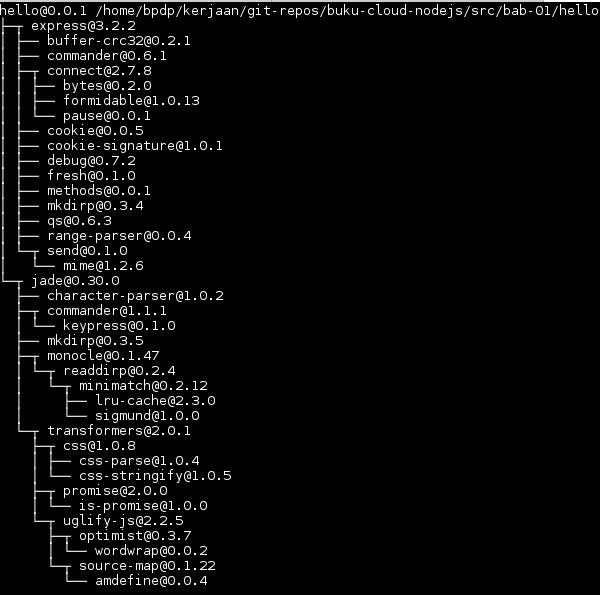
\includegraphics[scale=0.5]{images/npm-ls-paket-terinstall.jpg}
    \end{center}
    \caption{Tampilan ``npm ls'' pada direktori proyek dengan paket terinstall lengkap}
    \label{fig:npm-ls-paket-terinstall}
  \end{figure}

\subsection{Menghapus Paket / \textit{Uninstall}}

\index{npm!Hapus paket}Menghapus paket pustaka menggunakan npm pada dasarnya hampir sama dengan saat memasang paket, namun dengan perintah \textit{uninstall}. Berikut perintah lengkapnya.

\lstset{language=bash,caption=Perintah menghapus paket di npm}
\lstinputlisting{src/non-nodejs/bab-04/npm-uninstall.txt}

\subsection{Mencari Paket}

\index{npm!Cari paket}Untuk mencari paket, gunakan argumen \textit{search} dan nama atau bagian dari nama paket yang dicari. Contoh berikut ini akan mencari paket dengan kata kunci 'sha512' (tampilan berikut merupakan tampilan yang terpotong):

\lstset{language=bash,caption=Perintah menghapus paket di npm}
\lstinputlisting{src/non-nodejs/bab-04/npm-search.txt}

Setelah menemukan paketnya, pemrogram bisa menginstall langsung ataupun melihat informasi lebih lanjut tentang pustakan tersebut.

\subsection{Menampilkan Informasi Paket}

\index{npm!Info paket}Setelah mengetahui nama paket, pemrogram bisa memperoleh informasi lebih lanjut dalam format JSON menggunakan parameter \textit{view}. Contoh dibawah ini menampilkan rincian dalam format JSON dari paket \textit{arango.client}:

\lstset{language=bash,caption=Menampilkan rincian suatu paket dalam format JSON}
\lstinputlisting{src/non-nodejs/bab-04/npm-view.txt}

\subsection{Memperbaharui Paket}

\index{npm!Update paket}Jika terdapat versi baru, kita bisa memperbaharui secara otomatis menggunakan argumen \textit{update} berikut ini:

\lstset{language=bash,caption=Memperbaharui paket}
\lstinputlisting{src/non-nodejs/bab-04/npm-update.txt}
